% ============================================================================
% Point hebdomadaire -- Modelisation de l'accessibilite des geosites, Maroc
% GSMI, UM6P
% ============================================================================
\documentclass[11pt,aspectratio=169]{beamer}

\usepackage[utf8]{inputenc}
\usepackage[T1]{fontenc}
\usepackage[french]{babel}
\usepackage{newpxtext}
\usepackage{newpxmath}
\usepackage{booktabs}
\usepackage{array}
\usepackage{graphicx}
\usepackage{tikz}

\definecolor{accent}{HTML}{2B5F72}
\definecolor{accentlight}{HTML}{E7EEF2}
\definecolor{highlight}{HTML}{C9782E}
\definecolor{darktext}{HTML}{2B2B2B}
\definecolor{graytext}{HTML}{6B6B6B}

% ---------------------------------------------------------------- Theme ----
\usetheme{default}
\useoutertheme{infolines}
\useinnertheme{rectangles}
\setbeamertemplate{navigation symbols}{}
\setbeamercolor{normal text}{fg=darktext}
\setbeamercolor{structure}{fg=accent}
\setbeamercolor{frametitle}{fg=accent, bg=white}
\setbeamercolor{title}{fg=accent}
\setbeamercolor{footline}{fg=graytext, bg=white}
\setbeamercolor{page number in head/foot}{fg=graytext}
\setbeamerfont{frametitle}{series=\bfseries, size=\Large}
\setbeamerfont{footline}{size=\tiny}
\setbeamertemplate{itemize item}{\color{accent}\textbullet}
\setbeamertemplate{itemize subitem}{\color{highlight}\textendash}

\setbeamertemplate{headline}{}
\setbeamertemplate{footline}{%
  \leavevmode
  \hbox{%
    \begin{beamercolorbox}[wd=.62\paperwidth,ht=2.6ex,dp=1.2ex,leftskip=0.4cm]{footline}
      \usebeamerfont{footline}\color{graytext}\textit{GSMI -- Mod\'elisation de l'accessibilit\'e des g\'eosites}
    \end{beamercolorbox}%
    \begin{beamercolorbox}[wd=.38\paperwidth,ht=2.6ex,dp=1.2ex,rightskip=0.4cm,right]{footline}
      \usebeamerfont{footline}\color{graytext}\insertframenumber\,/\,\inserttotalframenumber
    \end{beamercolorbox}}%
  \vskip 0pt
}
\setbeamertemplate{frametitle}{%
  \vspace{0.15cm}
  \hspace{0.4cm}\insertframetitle\\[2pt]
  \hspace{0.4cm}\color{accent!30}\rule{0.94\paperwidth}{0.9pt}
  \vspace{0.1cm}
}

\newcommand{\source}[1]{{\tiny\color{graytext}#1}}

\title{Mod\'elisation de l'accessibilit\'e des g\'eosites au Maroc}
\date{Ao\^ut 2026}

\begin{document}

% ============================================================ Titre =======
{
\setbeamertemplate{footline}{}
\begin{frame}[plain]
  \centering
  
\includegraphics[width=0.34\linewidth]{../report/um6p_figures/um6p_gsmi_logo.png}\\[0.9cm]
  {\color{accent!35}\rule{0.32\linewidth}{0.5pt}}\\[0.9cm]
  {\Large\bfseries\color{accent} Mod\'elisation de l'accessibilit\'e des g\'eosites au Maroc}\\[0.35cm]
  {\normalsize\color{darktext} Point hebdomadaire : nouvelle base de donn\'ees, r\'esultats finaux, finalisation du rapport}\\[0.9cm]
  {\footnotesize\itshape\color{graytext} Geology and Sustainable Mining Institute (GSMI), UM6P}\\[0.6cm]
  {\footnotesize\color{graytext} Ao\^ut 2026}
\end{frame}
}

% ============================================================ Plan ========
\begin{frame}{Plan}
  \begin{enumerate}
    \setlength\itemsep{0.5em}
    \item Contexte : de l'ancien catalogue \`a la nouvelle base
    \item M\'ethodologie finale
    \item R\'esultats principaux
    \item Cartes : ce que chacune montre
    \item Limites de g\'en\'eralisation inter-r\'egions
  \end{enumerate}
\end{frame}

% ============================================================ Contexte ====
\begin{frame}{Contexte : de l'ancien catalogue \`a la nouvelle base}
  \begin{itemize}
    \setlength\itemsep{0.8em}
    \item Avant : \textbf{324} g\'eosites catalogu\'es, dont \textbf{251} \'etiquet\'es (77,5\,\%)
    \item Maintenant : \textbf{1\,154} g\'eosites catalogu\'es, dont \textbf{733} \'etiquet\'es
    \item Avant d'exploiter ce catalogue \'elargi, v\'erification que la taille seule
      n'expliquait pas un gain de pr\'ecision : cinq familles de mod\`eles diff\'erentes
      test\'ees sous le m\^eme protocole de validation -- aucune n'a d\'epass\'e
      l'ensemble d'arbres de mani\`ere significative, confirmant un plafond li\'e aux
      variables disponibles, pas au choix d'algorithme
  \end{itemize}
  \vfill
  \source{Source : archive/report\_old (catalogue initial) ; Table 1 et r\'esultats de
  validation crois\'ee du rapport actuel (catalogue actuel).}
\end{frame}

% ============================================================ Methodologie
\begin{frame}{M\'ethodologie finale}
  \begin{itemize}
    \setlength\itemsep{0.9em}
    \item \textbf{Variables} : pente, rugosit\'e, \'elévation, distance \`a la route,
      distance aux localit\'es, friction d'occupation du sol (LULC) -- six au total
    \item \textbf{Mod\`eles test\'es} : r\'egression logistique, $k$-NN (distance
      g\'eographique), $k$-NN (distance dans l'espace des variables), Processus
      Gaussien, ensemble d'arbres -- \textbf{mod\`ele retenu : l'ensemble d'arbres}
      (Random Forest + XGBoost + Gradient Boosting + LightGBM)
    \item \textbf{Validation} : validation crois\'ee LOGO par cluster de 500\,m,
      validation \guillemotleft\,leave-region-out\,\guillemotright, et validation par
      blocs spatiaux pour le mod\`ele de favorabilit\'e
  \end{itemize}
\end{frame}

% ============================================================ Resultats ===
\begin{frame}{R\'esultats principaux}
  \vspace{0.2cm}
  \begin{center}
  \small
  \begin{tabular}{@{}>{\raggedright\arraybackslash}p{4.8cm}r>{\raggedright\arraybackslash}p{3.6cm}>{\raggedright\arraybackslash}p{2.4cm}r@{}}
    \toprule
    Mod\`ele & $N$ & M\'ethode de validation & M\'etrique & Valeur (\%) \\
    \midrule
    Eddakhla (Difficile vs.\ non) & 25 & Leave-region-out & Exactitude & 96,0 \\
    Favorabilit\'e des g\'eosites & 1\,154 & CV par blocs spatiaux & AUC & 92,7 \\
    F\'es-Mekn\'es (Facile vs.\ non) & 322 & LOGO-cluster & Exactitude & 78,6 \\
    B\'eni Mellal-Kh\'enifra (Facile vs.\ non) & 157 & LOGO-cluster & Exactitude & 77,7 \\
    National (Difficile vs.\ non) & 733 & LOGO-cluster & Exactitude & 74,1 \\
    National (Facile vs.\ non) & 733 & LOGO-cluster & Exactitude & 73,3 \\
    \bottomrule
  \end{tabular}
  \end{center}
  \vfill
  \source{Table 3 du rapport. LOGO-cluster = validation crois\'ee \guillemotleft\,leave-one-group-out\,\guillemotright\ par cluster haversine de 500\,m.}
\end{frame}

% ============================================================ Cartes ======
\begin{frame}{V\'erit\'e terrain : 733 g\'eosites, classe r\'eelle}
  \centering
  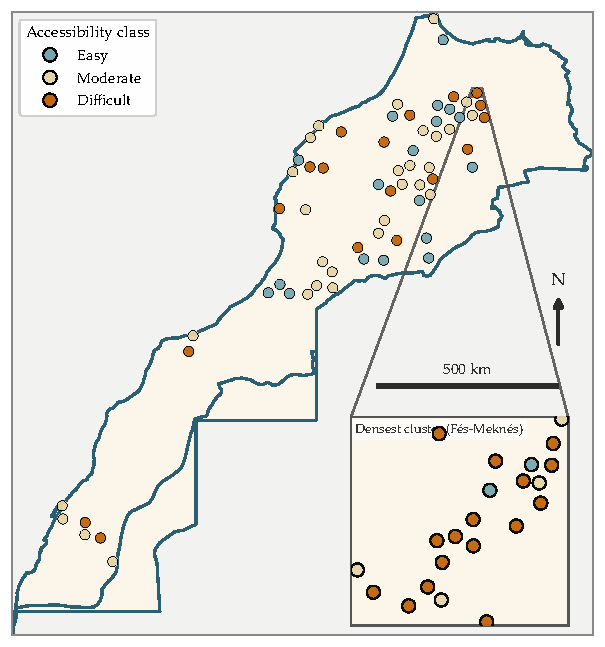
\includegraphics[height=5.1cm]{../report/figures/map_groundtruth_national.pdf}
  \vfill
  \source{Les g\'eosites \'etiquet\'es se concentrent dans le corridor Moyen Atlas /
  F\'es-Mekn\'es ; les sites Difficiles se concentrent le long du Rif et du front du
  Moyen Atlas.}
\end{frame}

\begin{frame}{Cas le plus favorable : Eddakhla-Oued Eddahab}
  \centering
  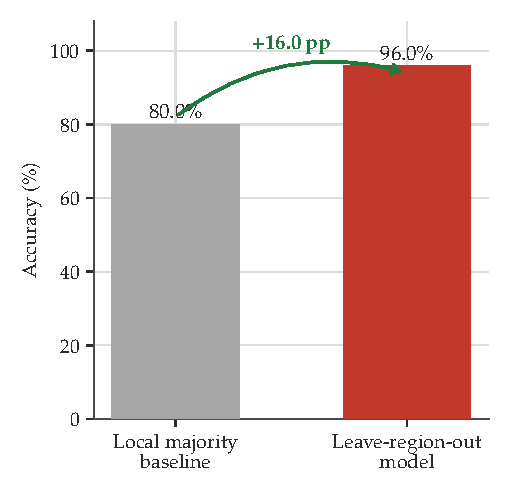
\includegraphics[height=4.8cm]{../report/figures/eddakhla_hero.pdf}%
  \hspace{0.4cm}%
  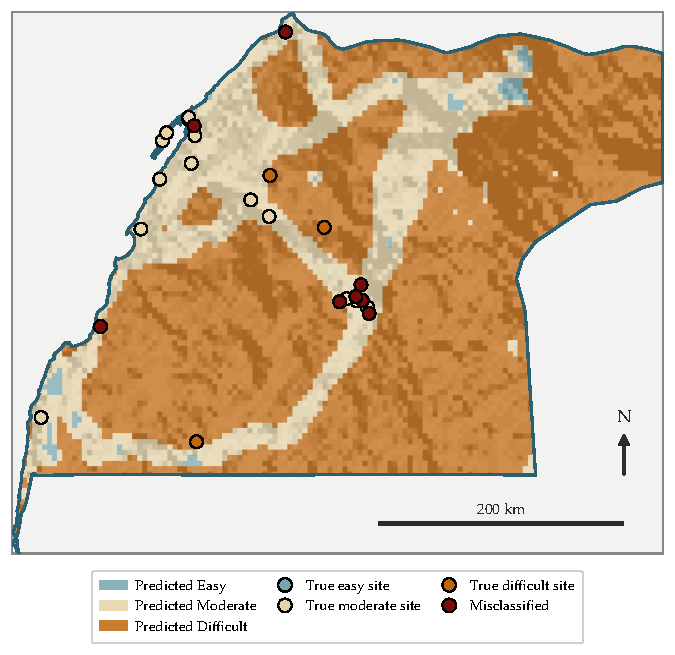
\includegraphics[height=4.8cm]{../report/figures/map_eddakhla.pdf}
  \vfill
  \source{Leave-region-out : entra\^in\'e sur les dix autres r\'egions uniquement,
  test\'e sur les 25 sites d'Eddakhla en totalit\'e. 96,0\,\% contre une base de
  80,0\,\% (classe majoritaire locale).}
\end{frame}

\begin{frame}{\'Etudes de cas r\'egionales}
  \centering
  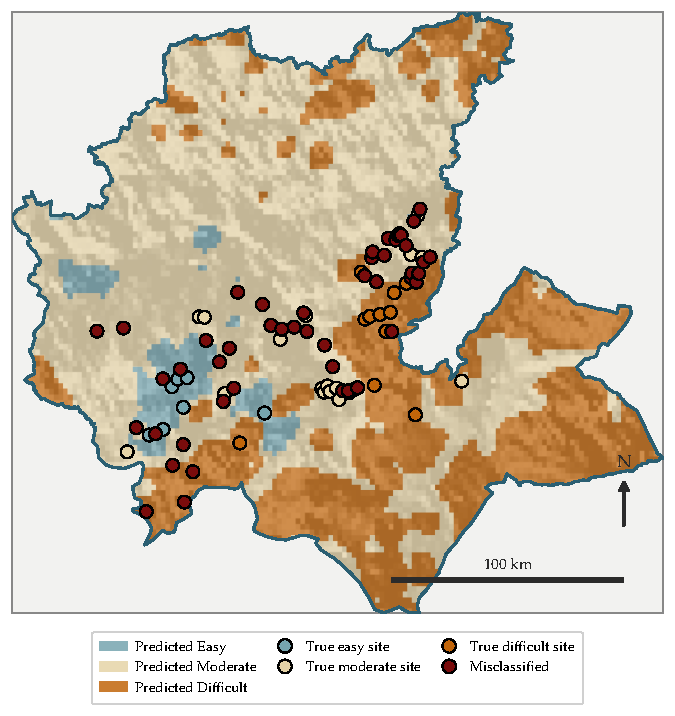
\includegraphics[height=5.0cm]{../report/figures/map_fesmeknes.pdf}%
  \hspace{0.3cm}%
  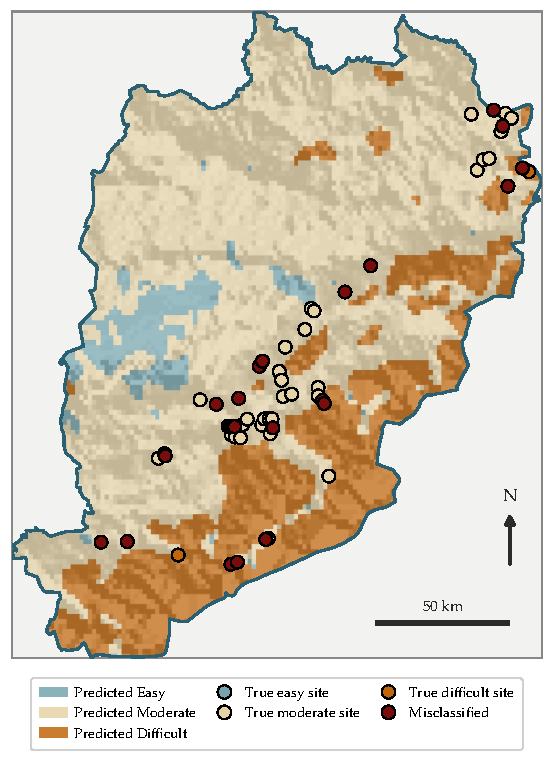
\includegraphics[height=5.0cm]{../report/figures/map_bmk.pdf}
  \vfill
  \source{Chaque carte provient d'un classificateur entra\^in\'e et valid\'e
  uniquement sur les donn\'ees propres \`a cette r\'egion, pas du mod\`ele national
  group\'e.}
\end{frame}

\begin{frame}{\'Echelle nationale et favorabilit\'e des g\'eosites}
  \centering
  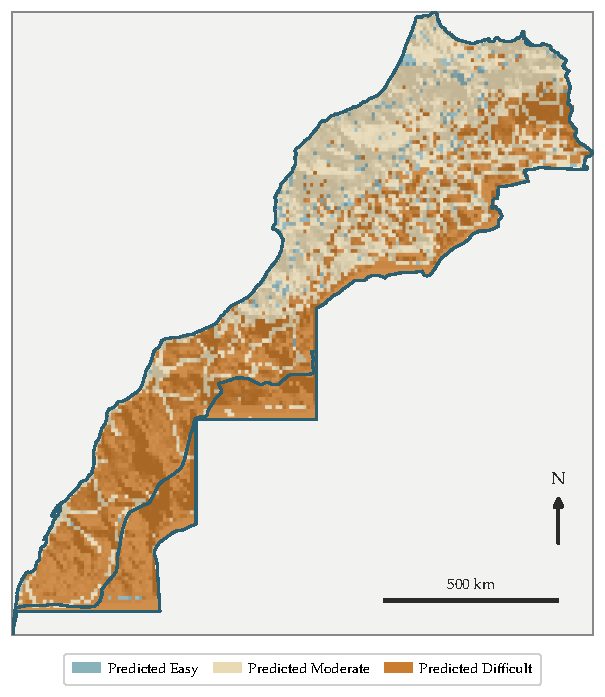
\includegraphics[height=5.0cm]{../report/figures/map_national.pdf}%
  \hspace{0.3cm}%
  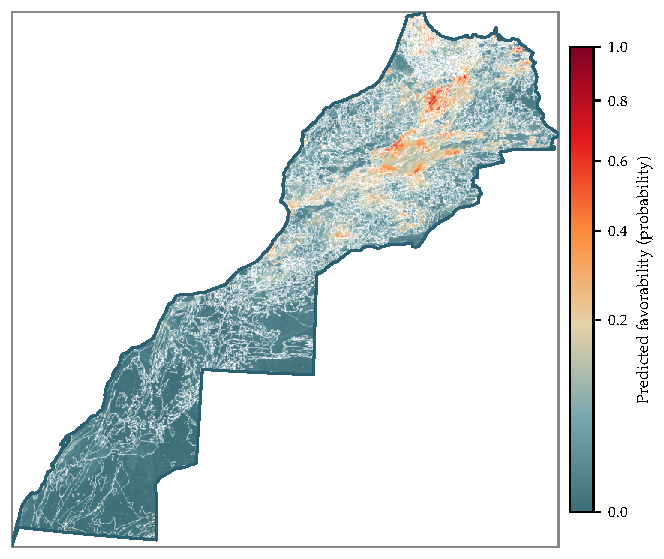
\includegraphics[height=5.0cm]{../report/figures/map_favorability.pdf}
  \vfill
  \source{\`A gauche : mod\`ele group\'e sur les onze r\'egions (74,1\,\%/73,3\,\%).
  \`A droite : un mod\`ele distinct r\'epondant \`a une autre question -- \emph{o\`u}
  se trouvent probablement des g\'eosites, plut\^ot que la difficult\'e d'acc\`es d'un
  site connu (AUC 0,927).}
\end{frame}

% ============================================================ LRO limits ==
\begin{frame}{Limites de g\'en\'eralisation inter-r\'egions}
  \centering
  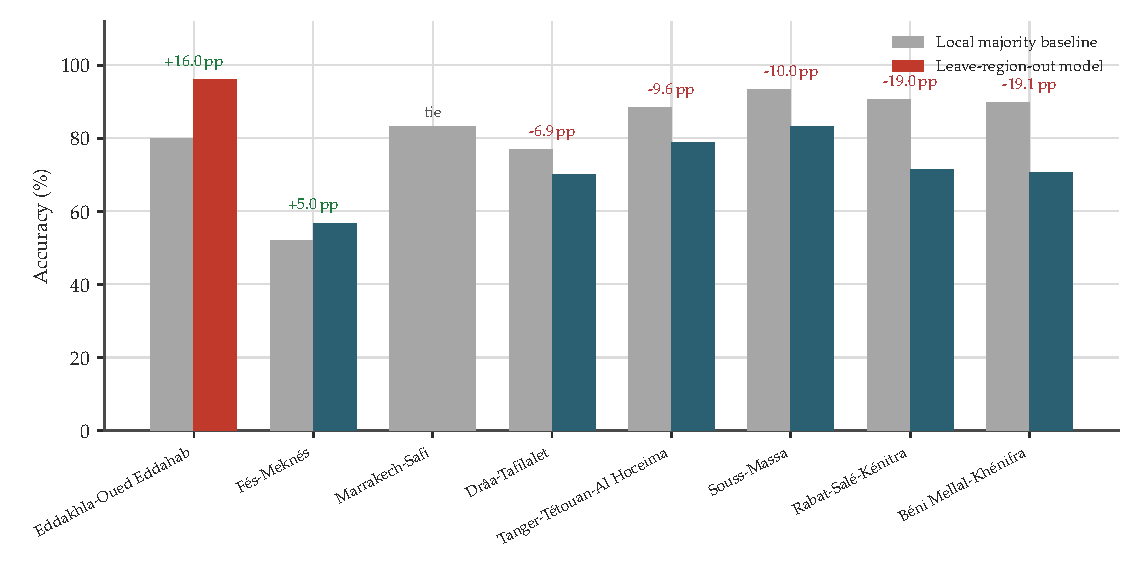
\includegraphics[height=3.1cm]{../report/figures/leave_region_out.pdf}

  \vspace{0.1cm}
  \scriptsize
  \begin{itemize}
    \setlength\itemsep{0.12em}
    \item \textbf{Eddakhla} (+16,0\,pts) : relief plat et homog\`ene, un seul facteur
      domine (distance \`a la route) -- terrain le plus facile \`a g\'en\'eraliser
    \item \textbf{F\'es-Mekn\'es} (+5,0\,pts) : \'echantillon le plus large (N=322),
      ce qui favorise la g\'en\'eralisation
    \item \textbf{B\'eni Mellal-Kh\'enifra} (-19,1\,pts) et \textbf{Dr\^aa-Tafilalet}
      (-6,9\,pts) : trop peu de sites \guillemotleft\,Difficile\,\guillemotright\
      (16 et 20) pour un mod\`ele fiable ; BMK combine en plus deux reliefs tr\`es
      diff\'erents (Haut Atlas et plaine du Tadla)
    \item \textbf{Tanger-T\'etouan-Al Hoceima} (-9,6), \textbf{Souss-Massa} (-10,0),
      \textbf{Rabat-Sal\'e-K\'enitra} (-19,0) : \'echantillons trop petits
      (21 \`a 52 sites) pour apprendre un motif transf\'erable
  \end{itemize}
  \vfill
  \source{\'Ecarts par rapport \`a la base de classe majoritaire locale, classificateur
  Difficile, leave-region-out (final\_v2\_results\_N733.json).}
\end{frame}

% ============================================================ Fin =========
{
\setbeamertemplate{footline}{}
\begin{frame}[plain]
  \centering
  \vspace{2cm}
  {\Large\bfseries\color{accent} Fin de la pr\'esentation}\\[0.4cm]
  {\normalsize\color{graytext} Questions et discussion}
\end{frame}
}

\end{document}
